\chapter{Testing and Evaluation}
\label{chapter:test-eval}

\section{Environment Setup}
\label{section:setup}

The development and testing of Open vSwitch can be done using many virtualization solutions. The
results presented here are based on using Mininet\cite{mn}. It is also possible to use some KVM\cite{kvm}
virtual machines. No matter of the chosen solution, the switch can connect to an
external controller or function independently as a learning switch. As a controller, we opted
to use a custom controller, written in Python, using the Ryu\cite{ryu} SDN framework.

Mininet contains a series of scripts capable of creating a virtualized network. It is simple to
use and provides a fast way to test various network protocols and solutions by creating
an entire network topology using virtualization containers. In this case, Open vSwitch will
be able to connect together the containers and can also be used with a controller.
Interaction with the system is done with an \texttt{API} or through a single command line console.
Commands are prefixed with the name of the host where the process should be run as shown in
Listing~\ref{lst:mn}.
\lstset{caption=Mininet Command Line,label=lst:mn}
\begin{lstlisting}
 mininet> h1 ping h2
 mininet> h1 ifconfig
\end{lstlisting}
Any Linux command can be used, provided that it is installed on the host.

Because we are working with new features of the OpenFlow protocol which are not implemented, some of
the initial development was done by simulating messages from a controller. It is a slow and difficult method
because it involves writing by hand the contents of the packets that we need our switch to process.
The \texttt{ovs-appctl} command was ran like shown in Listing~\ref{lst:manual-packet} to send packets
directly to Open vSwitch.

\lstset{caption=Manually Sending OpenFlow Messages,label=lst:manual-packet}
\begin{lstlisting}
 $ ovs-appctl -t ovs-ofctl ofctl/send "05 21 00 10 00 00 00 0a 00 00 00 01 00 02 00 01"
\end{lstlisting}

We later developed a tool called ovs-pktgen\footnote{\url{https://github.com/IxLabs/ovs-pktgen}}
to aid in the generation of OpenFlow messages by filling-in the fields of the actual on-the-wire
data structures. It extends the build scripts that already parse some header files to obtain the
data structure fields for each type of OpenFlow message supported by Open vSwitch. The user only
has to enter the version and message name. The fields are listed with the corresponding data type
and the contents is read from the terminal. At the end, the tool forms the entire OpenFlow message
and prints the hexadecimal representation of its contents.

After implementing other OpenFlow 1.4 features required for Open vSwitch to connect
to an OpenFlow 1.4 controller, we were able to use Mininet with our own custom controller.

Basically, our environment is setup by issuing the commands shown in Listing~\ref{lst:setup}.
\lstset{caption=Setting up the Development Environment,label=lst:setup}
\begin{lstlisting}
 # ovsd-server [...] &
 # ovs-vswitchd [...] &
 # ryu-manager ryu-switch-port-mod.py &
 # mn --controller=remote,ip=127.0.0.1
\end{lstlisting}
The first two lines are required to start up Open vSwitch and they need various other parameters.
Then, the controller built with the Ryu framework is started and, finally, Mininet will tie
everything together by configuring Open vSwitch to use the controller that was previously started.

Another testing environment used is a set of 2 KVM virtual machines. These are configured to
boot a Linux kernel and mount the host's file system, similar to the testing environment that
I used in my previous research. This solution is better when one is also testing kernel related
aspects in one of the VMs. We used this setup for developing the security application presented
in Chapter~\ref{chapter:app}.

\section{Results}

\subsection{Open vSwitch Hackathon}

An Open vSwitch hackathon\footnote{\url{http://openvswitch.org/pipermail/announce/2013-August/000053.html}}
was the first opportunity we had to gain more experience about the project
and to start contributing fixes and features. It was held on 6 - 7 September, 2013 and the main
purpose was to improve the support for OpenFlow in Open vSwitch. By the end of the hackathon we managed
to add a missing OpenFlow 1.3 functionality, processing \texttt{GET_ASYNC_CONFIG} messages.

The handling of the \texttt{ROLE_STATUS} OpenFlow messages was successfully integrated\footnote{\url{http://openvswitch.org/pipermail/git/2013-October/004800.html}}
into Open vSwitch, one month after the hackathon.
In order to test the functionality and prevent future regressions, some unit tests
where also implemented. The Open vSwitch project already has a set of tests for probably
any functionality. These are written using GNU Autotest from the Autoconf\cite{autoconf}
package by sending custom messages to the switch, simulating a controller.

\subsection{OpenFlow Bundles}

The implemented interface for bundles from the specification works as expected. The corner cases also
have unit tests, like the one in Appending~\ref{lst:test-bundles}. This forms a base for implementing batching messages of any types. This part
of the project is already included in the upstream Open vSwitch. The main series of patches was
accepted after 6 iterations and reviews.

We have complete support for batching together multiple port-mod messages in bundles. Currently,
we are getting feedback on how to properly integrate the feature in Open vSwitch.

OpenFlow flow-mod messages are also permitted in bundles, but the implementation is not complete.
We only support adding and removing flow messages.


\section{Evaluation}

In order to determine the performance of the OpenFlow bundles implementation, a comparative test
was created. The learning switch controller was modified to create bundles, add messages to them
and then commit the bundle. We recorded the running time of these operations on the controller side.
The results were then compared with the running time for the same messages sent to the controller,
but without using bundles. All tests were run $5$ times and the results were averaged.

The tests were run with $100000$ port-mod messages, using an increasing number of ports connected to a single
switch. The results in Table~\ref{tbl:bundleperf} show that the duration of the commit operation is constant,
regardless of the number of ports. The total duration for processing bundled messages is, on average,
$36\%$ slower than sending each message individually. This also includes the duration for allocating
a bundle and closing it.

It can also be observed that the total number of ports in the switch does not influence the performance.
In this case, each port-mod message in a bundle is referring to a single port of the switch. Therefore, the
list of modified ports has only one element which is accessed in constant time.

\begin{table}[h]
  \centering
  \begin{tabular}{rrrrr}
    \toprule
      Port Count & Individual Message Time(ms) & Bundled Message Time(ms) & Commit time(ms) \\
    \midrule
        2 & 3624 & 5091 & 0.016 \\
       10 & 3573 & 4814 & 0.016 \\
       100 & 3697 & 4961 & 0.016 \\
    \bottomrule
  \end{tabular}
  \caption{Bundled Messages Performance for 100000 Messages}
    \label{tbl:bundleperf}
\end{table}

We also ran the same tests by equally distributing the ports to the $100000$ port-mod messages. The results
are shown in Table~\ref{tbl:bundleperf2}. In this case, the relative performance drop is, on average, of only $32\%$.
The two sets of results are almost identical. One explanation is that the number of messages and the number of
ports is relatively small. We believe that even with larger number of ports the performance doesn't degrade
to the point of becoming a problem. Moreover, these results were obtained by having the switch and the controller
on the same physical machine. If the controller was to run in another network, or even in the local network
and with a smaller number of messages, the difference in processing time would be on the same level as the network latency.

\begin{table}[h]
  \centering
  \begin{tabular}{rrrrr}
    \toprule
      Port Count & Individual Message Time(ms) & Bundled Message Time(ms) & Commit time(ms) \\
    \midrule
        2 & 3584 & 4752 & 0.015 \\
       10 & 3589 & 4778 & 0.015 \\
       100 & 3651 & 4888 & 0.015 \\
    \bottomrule
  \end{tabular}
  \caption{Bundled Messages Performance for 100000 Messages and Different Ports}
    \label{tbl:bundleperf2}
\end{table}

We can better observe the performance implications of using OpenFlow bundles in Figure~\ref{fig:bundleperf}.
A similar test was run with bundles of flow-mod messages and the same performance penalty of $31\%$ was observed.
This is also an indication that the controller itself has an overhead included in these results. Knowing that
our implementation for flow-mod messages in bundles has a slow path in the commit phase, and the commit duration
is the same like it is for port-mod messages, we can conclude that the actual decapsulation and pre-processing
of the packets is the most time consuming task.

\begin{figure}[h]
  \begin{center}
    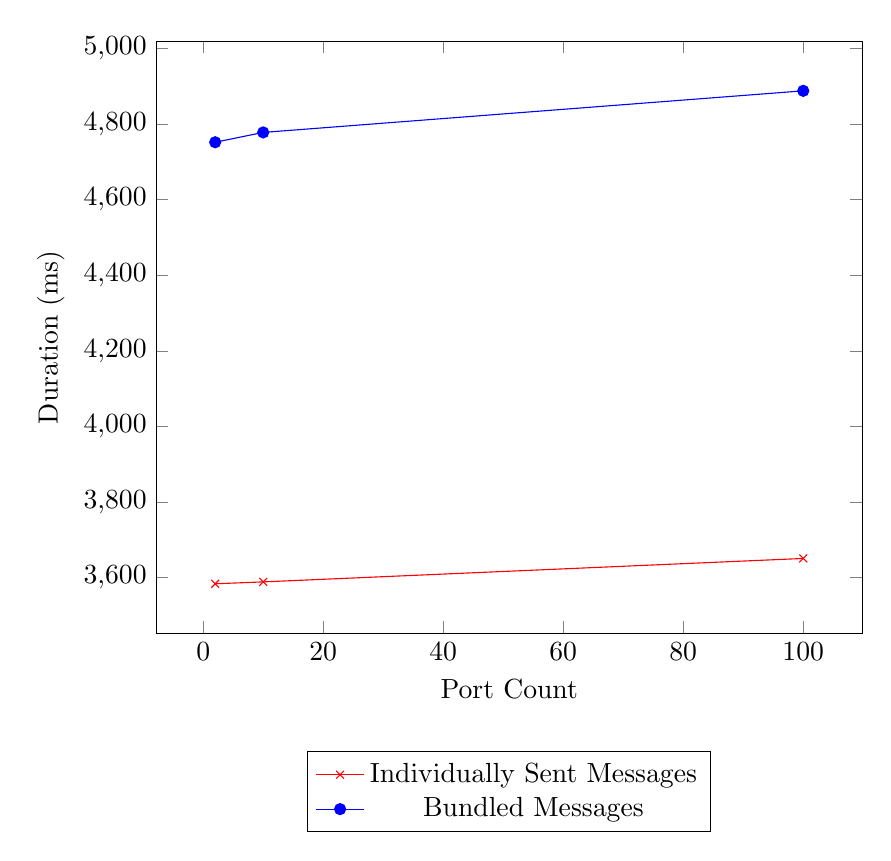
\begin{tikzpicture}
	    \begin{axis}[
		    xlabel=Port Count,
		    ylabel=Duration (ms),
		    legend style={at={(0.5,-0.20)},anchor=north},
		    width=300
		    ]
	    \addplot[sharp plot,color=red,mark=x] coordinates {
		    (2,3584)
		    (10,3589)
		    (100,3651)
	    };
	    \addplot[sharp plot,color=blue,mark=*] coordinates {
		    (2,4752)
		    (10,4778)
		    (100,4888)
	    };
	    \legend{Individually Sent Messages, Bundled Messages}
	    \end{axis}
    \end{tikzpicture}
    \caption{Bundled Messages Performance for 100000 Messages}
    \label{fig:bundleperf}
  \end{center}
\end{figure}
